\documentclass[a4paper]{IEEEtran}

\usepackage[latin1]{inputenc}
\usepackage{epstopdf}
%\usepackage[spanish]{babel}
\usepackage[cmex10]{amsmath}
\interdisplaylinepenalty=2500
\usepackage{amsfonts}
\usepackage{amssymb}
\usepackage{graphicx}
\usepackage{verbatim}
\usepackage{array}
\usepackage{multirow}
\usepackage{dcolumn}
\usepackage{color}
\usepackage[noadjust]{cite}
\usepackage{url}
\usepackage{balance}
\usepackage[usenames,dvipsnames]{xcolor}
\usepackage{accents}
\DeclareGraphicsExtensions{.eps}
\AppendGraphicsExtensions{.pdf}

\DeclareMathOperator*{\Max}{max}
\DeclareMathOperator*{\Min}{min}
\DeclareMathOperator*{\argmin}{arg\,min}
\DeclareMathOperator*{\Maximize}{Maximize}

\begin{document}
\title{Risk- and Ambiguity-Constrained Renewable Portfolio Model with Call Options}

\author{Bruno~Fanzeres,~\IEEEmembership{Student Member,~IEEE,}
		Arthur~Brigatto,~\IEEEmembership{Student Member,~IEEE,}
	    Alexandre~Street,~\IEEEmembership{Member,~IEEE,}	
        and Luiz~Augusto~Barroso,~\IEEEmembership{Senior Member,~IEEE}

%\thanks{This work was partially supported by UTE Parna\'iba Gera\c{c}\~ao de Energia S.A. through R\&D project ANEEL PD-7625-0001/2013.}
%\thanks{Bruno Fanzeres, Arthur Brigatto and Alexandre Street are with the Electrical Engineering Department, Pontifical Catholic University of Rio de Janeiro (PUC-Rio), Rio de Janeiro, RJ, Brazil (e-mail: \mbox{bsantos@ele.puc-rio.br}; \mbox{street@ele.puc-rio.br}).}
%\thanks{L. A. Barroso are with PSR Consulting, Rio de Janeiro, RJ, Brazil (e-mail: \mbox{luiz@psr-inc.com}).}
}

\maketitle
\begin{abstract}
	Within competitive electricity markets, supply contracts plays an important role. They help ensure supply adequacy and mitigate market power, among other benefits. However, when renewable energy is involved, the mixture of an uncertain energy production with a high volatile short-term market poses a risk difficult to manage. Within this context, call options are suitable hedging instruments due to the right to purchase relatively cheap energy to cover renewable unbalances (with respect to supply contracts) in periods of spot price spikes. To efficiently balance the cost/benefit of a set of call options in a portfolio of renewable sources short in supply contracts, a precise definition of the probabilistic nature of the short-term market price should be available. However, it is recognized that in practice agents only have an imprecise approximation of the ``true'' underlying process. Thus, decisions are made under \textit{ambiguity}. Therefore, the standard pure stochastic approach for optimal composition of electricity contracts may not be suitable. In this work, we propose a risk and ambiguity-adjusted portfolio allocation model that defines the optimal composition of call options and renewable sources to back a forward contract. A case study with real data from the Brazilian power system is presented.
\end{abstract}

\begin{IEEEkeywords}
	Ambiguity constraints, call options, conditional value-at-risk, multi-level programming, power system economics, renewable energy, forward contract.
\end{IEEEkeywords}

% ===== Sec. I - Introduction ===== %

\section{Introduction}
\label{Introduction}

	\IEEEPARstart{T}{he} introduction of competitiveness in generation sector of most power systems around the world altered the way that Energy Trading Companies (ETCs) act in energy markets. Investments in new power plants are no longer driven by load growth, but by the search of an adequate balance between expected future profit and risk exposure. Furthermore, short-term energy trading and contract portfolio management became a relevant routine in most ETC's everyday activities. In this framework, a key challenge in decentralized markets relies on the determination of a set of investments and optimal contracting/bidding strategies that creates maximum value for electricity agents, taking into account several sources of uncertainties inherent to the business, such as energy, gas and fuel prices, as well as equipment deficiency, regulatory changes, failure in transmission lines, among others. In addition, when renewable sources are involved, their uncertain production is also a risk factor that must be considered in the decision problem \cite{RiskConstPortSelect}.

	Since the beginning of the deregulation process, several works have discussed methods to manage uncertainty on energy trading. One of the approaches widely adopted by practitioners is the acquisition of hedging instruments to protect their cash flow against unexpected events. In practice, there are two instruments commonly negotiated: forward contracts and options. Forward contracts are known to provide adequate hedge for thermal units against spot price volatility, which induces the so-called \textit{price risk} \cite{HedgingQtdRisk_Oren}. Their controlled self-generation prevents energy purchase in short-term markets at undesirable levels to fulfill the delivery obligation. However, in the case of renewable units -- such as hydro and wind plants -- the probabilistic and seasonal nature of their physical production induces an additional risk for the electricity company, the \textit{volume risk} \cite{HedgingQtdRisk_Oren}, which happens whenever the (stochastic) volume of energy produced is not sufficient to meet contract obligations and the company must buy the difference on highly volatile short-term market. Therefore, in addition to forward contracts, ETCs acquire different types of options with the objective of mitigating the joint price and volume risk associated with scenarios of energy unbalance and high spot price. In this context, a major challenge that energy companies face on competitive markets lie in the definition of the optimal mix between renewable portfolio and hedge instruments to be contracted through a co-optimization model.

	The problem of optimal portfolio allocation of electricity contracts has been widely studied in different contexts and market structures. Typically, the mathematical modeling starts with the identification of the uncertainty factors that affect the portfolio, e.g. renewable production and energy spot price. Then, a probabilistic description of these uncertainties is defined under the form of joint distribution functions or econometric/time-series models. Finally, a stochastic optimization problem that specifies the optimal portfolio of contracts to be settled is constructed. To solve such optimization problem, practitioners usually sample a set of ``scenarios'' (possible realizations) for the uncertainty factors from the available probability description and solve an approximate stochastic programming problem \cite{Birge_StochProgm}. A key point on implementing such modeling in the context of energy trading is to assess an accurate description of the probabilistic nature of the short-term market price. It is recognized that in practice agents only have an imprecise estimation of the ``true'' underlying process that guide the future spot price behavior. In addition, in the presence of severe price movements, this modeling error is worsened, which ultimately lead to non recoverable financial losses. Given this high difficulty on uncertainty characterization, decision makers act under \textit{ambiguity} and intuitively adjust their preferences over stochastic cash flows toward the ones derived from portfolios obtained under adverse conditions. Most of these agents follow a max-min structure where the optimal portfolio is constructed with the worst-possible realization of the uncertain parameters for the decision maker objectives \cite{SoftRobustModel_UnderAmb}. 

	Therefore, the main objective of this work is to devise an unified risk and ambiguity-constrained electricity portfolio allocation model of renewable, forward and call option contracts. Specifically, from a commercial point-of-view, we extend the business model proposed in \cite{RobustSpotPrice} to include the possibility of purchase call options to adequately hedge a portfolio of renewable sources against the price and volume risk induced by the sale of a forward contract. On the other hand, from the point-of-view of decision structure and preference relation, we propose an extension of the classical risk-constrained portfolio selection model introduced by Markowitz \cite{PortSelect_Markovitz} and commonly used on energy markets \cite{RiskConstPortSelect} to include the decision maker aversion to uncertainty on the probability modeling. For this purpose, we adapt the hybrid stochastic/robust methodology developed in \cite{RobustSpotPrice, AmbiguityEnergySpotPrice} to construct a set of constraints that restricts the business profit to a pre-specified level under the worst possible realization of the short-term market price. As discussed in \cite{AmbiguityEnergySpotPrice}, this modeling approach possesses a one-to-one relation to a set of probability distributions of the energy spot price. Thus, the constraints imposed by the hybrid stochastic/robust methodology, which we call \textit{ambiguity constraints}, performs a worst-case analysis over a set of probability distributions. Such approach is widely used in ambiguity theory \cite{SoftRobustModel_UnderAmb} to handle uncertainty on probability modeling. It is noteworthy that, although the presence of call options in the portfolio helps to mitigate the price and volume risk faced by the ETC, their proper value is highly dependent on the accuracy of the short-term price probability description. Therefore, in the context of modeling uncertainty, the classical risk-constrained allocation approach widely used to compose an ``optimal'' portfolio may provide a significant suboptimal portfolio, exposing the agent to unexpected financial losses. Thus, we argue that the proposed approach, which devises a risk and ambiguity-averse portfolio, provides a significant improvement on assessing the benefits of call options in price and quantity risk mitigation.

\subsection{Contributions Regarding the Existing Literature}

	Several works appear in recent technical literature that tackle the challenges of the optimal trading of energy in deregulated markets. Here, we provide close related works of the many references in energy trading in order to contextualize the contributions of this paper. In \cite{AStochDMFram_ElectrRetailer}, a stochastic portfolio optimization model for a retailer that defines the optimal involvement in supply sources to procure its demand is proposed. Also, \cite{HedgingQtdRisk_Oren} explores the typical correlation between energy spot price and load demand to derive an optimal zero-cost hedging function that maximizes the agent's expected utility and discusses a methodology to construct a portfolio of forward and option contracts that replicate the hedging payoff in a single-period setting. Similarly to the business structure considered in this work, \cite{ManagFinRiskWithCall} presents a three-stage stochastic optimization model to determine the optimal selling strategy, including options, forward contracts and pool trading, of a risk-averse price-taker thermal unit. In addition, \cite{RiskConstPortSelect} propose a risk-constrained allocation model to define the optimal mix of small hydro and biomass sources to back a supply contract in hydrothermal markets. From a robust optimization perspective, \cite{OfferingStrat_RO} provides a technique to co-optimize the self-scheduling and hourly offering curves of a price-taker producer in which the standard short-term market price forecast is replaced by confidence intervals. In \cite{AmbiguityEnergySpotPrice}, an interesting relation between a robust max-min model and ambiguity theory is provided with application to renewable trading. Similarly, \cite{RobustSpotPrice} adapts the robust optimization approach to perform an endogenous stress test for spot prices in order to devise a portfolio of renewable sources and supply contracts.

	Following the main ideas exposed on these previously reported works, we propose a portfolio allocation model that aims to devise an optimal portfolio of renewable sources, forward contracts and call options in a risk and ambiguity-constrained framework. We refer to \cite{SoftRobustModel_UnderAmb} for an extensive theoretical discussion of a similar decision structure proposed in this work with applications to financial asset allocation. From a methodological view-point, our model fits in the class of single-stage robust linear optimization problems \cite{PriceOfRobustness}, requiring thus only basic linear programming algorithms to solve \cite{Xpress}. It is worth emphasizing that to the best of our knowledge no work has been reported on portfolio allocation of renewable energy with forward and call options in a risk and ambiguity-constrained setting. Therefore, the contributions of this paper are threefold:

	\begin{enumerate}
		\item to extend the business model presented in \cite{RobustSpotPrice, AmbiguityEnergySpotPrice} to include the trading of call options;
		\item to handle the imprecision on future spot price probability characterization by means of ambiguity risk constraints;
		\item to provide an efficient solution methodology for the proposed multilevel portfolio selection problem.
	\end{enumerate}

%\subsection{Organization of This Work}

%	\textcolor{red}{This paper is structured as follows: in Section \ref{ElectrContr}, the electricity contracts involved in this work are discussed and the trading revenue is derived. Section \ref{OptContrStrat} presents the uncertainty modeling considered and the proposed portfolio allocation model. In Section \ref{SolMeth}, the proposed solution methodology for the portfolio problem is presented. In section \ref{CaseStudy}, we present case studies with realistic data of the Brazilian power system. Finally, in Section \ref{Conclusions} we outline the conclusions and future work.}

% ===== Sec. II - Electricity Contract ===== %

\section{Electricity Contracts and Business Model}
\label{ElectrContr}

	The business environment here discussed involves the trading of three types of electricity arrangements: forward contracts with physical delivery obligation (supply contracts), capacity payment with renewable units and call options. It is assumed an ETC selling a supply contract to serve a firm load backed on renewable portfolio with the possibility to hedge the trading with call options. Throughout this work, we assume available a probability space $(\Omega, \mathcal{F}, \mathbb{P})$ with discrete sample space (plausible scenarios) where the random variables are defined \cite{Birge_StochProgm}. Additionally, for didactic purposes, we represent a random variable with an upper tilde (e.g. $\accentset{\sim}{\pi}$) and its realization in scenario $\omega \in \Omega$ as $\pi_{\omega}$. In the next subsections, we individually discuss each modality of contract and the role they play in this work. 

\subsection{Supply Contracts Backed on Renewable Generation}
\label{SupplyContract}

	Standard supply contracts are bilateral arrangements typically negotiated in electricity markets. They consist of an agreement to interchange a certain amount of energy $Q^{\text{sell}}$ (avgMW) during a specified time range at a price $P^{\text{sell}}$ (\$/MWh) \cite{RobustSpotPrice}. Specifically, the seller counterpart assumes full obligation to deliver the agreed energy in exchange of a fixed payment made by the buyer. Note that in this arrangement, the short-term risk is assumed by the seller since it has to buy in spot market the necessary energy to fulfill the contract. 

	A capacity (payment) contract is a modality of bilateral agreement which comprises energy coverage associated to a power source. Generally speaking, the buyer counterpart pays a fixed value to the underlying unit for the right to negotiate in the short-term market a percentage of its production, as a ``rent'' operation. In particular, when the unit involved is a renewable plant, the contract can be parametrized in two main variables: (i) a (fixed) price $P_{i}^{\text{res}}$ (\$/MWh) payed to the renewable generator for the respective (stochastic) energy production and (ii) a measure of ``firm energy'' $F_{i}^{\text{res}}$ (avgMW) associated to the unit. The idea behind a firm energy measure is to express the probabilistic nature of renewable production into a single value in order to quantify the amount of energy the producer is able to negotiate in the market \cite{SupplyAdequacy}. In this arrangement, the risk of short-term market exposure is transfered from the renewable producer to the contract buyer since the former receives a certain payment for its ``firm energy'' and the latter gains the right to negotiate in the short-term market the stochastic production of the renewable plant.

	Combining both contracts, the stochastic cash-flow of an ETC selling a supply contract backed by a set $U$ of renewable generators is presented next \cite{RobustSpotPrice}.
%
\begin{align}
	& R^{\text{supply}}_{t}(x^{\text{sell}}, \boldsymbol{x}^{\text{res}}, \accentset{\sim}{\pi}_{t}) = P^{\text{sell}} h_{t} Q^{\text{sell}} x^{\text{sell}} - \sum_{i \in U} P_{i}^{\text{res}} h_{t} F_{i}^{\text{res}} x_{i}^{\text{res}} \notag \\
	 		& \> \> \> \> \> \> \> \> \> \> + \Bigg( \sum_{i \in U} \accentset{\sim}{G}_{i,t}^{\text{res}} x_{i}^{\text{res}} - h_{t} Q^{\text{sell}} x^{\text{sell}} \Bigg)\accentset{\sim}{\pi}_{t}; \> \> \> \> \> \> \> \forall ~ t \in H, \label{RevSupplyCap}
\end{align}
%
where the first term represents a fixed supply payment received by the ETC, the second term indicates the fixed expenditure of each renewable generator in the portfolio and the third term stands for the short-term market settlement with $\accentset{\sim}{G}_{i,t}^{\text{res}}$ (MWh) and $\accentset{\sim}{\pi}_{t}$ (\$/MWh) the random variables representing the renewable production of the unit $i \in U$ and the energy spot price, respectively; $H$ defines the set of periods of the supply contract and $h_{t}$ the number of hours in period $t \in H$. In expression (\ref{RevSupplyCap}), $x^{\text{sell}}$ and $x_{i}^{\text{res}}$ represent, respectively, the percentage of energy sold in the supply contract and the percentage of each renewable source $i \in U$ brought to the portfolio. Note that this equation precisely reveals the price and volume risk faced by the ETC. For a given portfolio of renewable plants, if the ETC decides to fully sell the bilateral contract $(x^{\text{sell}} = 1)$, the fixed supply payment (first term of expression (\ref{RevSupplyCap})) is the highest possible. However, the energy unbalance exposure (third term of expression (\ref{RevSupplyCap})) and consequently the risk of purchase energy at high price levels in short-term market is also the highest possible. On the other hand, the decision to not sell the supply contract $(x^{\text{sell}} = 0)$ implies full renewable settlement in the short-term market, which is highly volatile \cite{SupplyAdequacy}.

\subsection{Call Options and the Business Revenue}

	With the intention of mitigating the price and volume risk discussed in section \ref{SupplyContract} we consider the possibility for the ETC to acquire European call options to hedge its portfolio. In the context of this work, a call option is a purely financial bilateral contract that gives the buyer (known as \textit{holder} of the option) the right, but not the obligation, to buy a certain amount of energy $Q_{j}^{\text{call}}$ (avgMW) at a specific time period for a fixed price $\Gamma_{j}^{\text{call}}$ (\$/MWh), called \textit{strike price}, defined \textit{a priori}. In exchange, the holder pays a fixed amount $P_{j}^{\text{call}}$ (\$/MWh), called option's \textit{premium}, to the contract seller (known as \textit{writer} of the option). The key point that makes energy call options a suitable hedge instrument against price and volume risk is the possibility to buy the agreed amount of energy at a known fixed price $\Gamma_{j}^{\text{call}}$. In other words, for scenarios $\omega \in \Omega$ of energy deficit and spot prices higher than the option's strike price, the buyer ``exercise'' the right to buy the agreed amount of energy at a fixed price level $\Gamma_{j}^{\text{call}} < \pi_{t,\omega}$ resulting in a payoff of $(\pi_{t,\omega} - \Gamma_{j}^{\text{call}})Q_{j}^{\text{call}} > 0$. On the other hand, for scenarios of spot prices below the strike price, there is no advantage in exercising the option, since energy can be bought at (relatively) low prices in the short-term market. Therefore, in the context of price and volume risk, call options are well-suited hedge instrument since they can efficiently cover the energy unbalance risk. Mathematically, for a given set $C_{t}$ of available call options in period $t \in H$, the stochastic cash-flow of a call option $j \in C_{t}$ is:
%
\begin{align}
	\hspace{-0.20cm} R_{j}^{\text{call}}(x_{j}^{\text{call}}, \accentset{\sim}{\pi}_{t}) = \Big( \text{max}\{0, \accentset{\sim}{\pi}_{t} - \Gamma_{j}^{\text{call}}\} - P_{j}^{\text{call}} \Big) h_{t} Q_{j}^{\text{call}} x_{j}^{\text{call}}. \label{CallCashFlow}
\end{align}

	The first term of (\ref{CallCashFlow}) reproduces the exercise rule discussed previously and the second term accounts for the premium paid to the option writer for the right embedded in the contract; $x_{j}^{\text{call}}$ defines the percentage of the $j \in C_{t}$ call option bought to hedge the portfolio. Expression (\ref{BusinessRevenue}) illustrates the resulting net revenue of an ETC during the whole business period by considering call options in the scheme described in section \ref{SupplyContract}.
%
\begin{align}
	& \hspace{-0.5cm} R(\mathbf{x}, \accentset{\sim}{\boldsymbol{\pi}}) = \sum_{t \in H} \Bigg[ P^{\text{sell}} h_{t} Q^{\text{sell}} x^{\text{sell}} - \sum_{i \in U} P_{i}^{\text{res}} h_{t} F_{i}^{\text{res}} x_{i}^{\text{res}} \notag \\
	 		& \> \> \> \> \> + \sum_{j \in C_{t}} \Big( \text{max}\{0, \accentset{\sim}{\pi}_{t} - \Gamma_{j}^{\text{call}}\} - P_{j}^{\text{call}} \Big) h_{t} Q_{j}^{\text{call}} x_{j}^{\text{call}} \notag \\
			& \> \> \> \> \> + \Bigg( \sum_{i \in U} \accentset{\sim}{G}_{i,t}^{\text{res}} x_{i}^{\text{res}} - h_{t} Q^{\text{sell}} x^{\text{sell}} \Bigg) \accentset{\sim}{\pi}_{t} \Bigg], \label{BusinessRevenue}
\end{align}
%
where $\mathbf{x} = [x^{\text{sell}}, \boldsymbol{x}^{\text{res}}, \boldsymbol{x}^{\text{call}}]^{\top}$. It is important to mention that the optimal composition of contracts should take into account the different characteristics and dynamics that each modality of contract holds and the synergy existent among them. For instance, the ETC must be aware of the tradeoff between the fixed payments (first and second terms of (\ref{BusinessRevenue})) and the price and volume risk introduced by the last term of (\ref{BusinessRevenue}) as well as the benefits of a portfolio of call options, balancing the cost incurred by the option's premium and the benefits in mitigating this risk. In the next section, we present the uncertainty characterization and the optimal portfolio allocation model proposed in this work.


% ===== Sec. III - Tri-Level Contracting Model ===== %

\section{The Risk and Ambiguity-Constrained Portfolio Allocation Model}
\label{OptContrStrat}

	In technical literature, there exist many different approaches to characterize the problem of portfolio selection under uncertainty. The classical one is the mean-variance approach introduced by Markowitz in his seminal work \cite{PortSelect_Markovitz}. The idea behind Markowitz's model is to compose a portfolio with the highest expected profit constraining the portfolio's risk to given a fixed level. A key point of this approach is the assumption that an accurate probability description of the uncertain parameters is available. However, in the context of energy trading, this assumption may not be met in practical applications due to the high difficulty on (precisely) characterizing the probability dynamics of the short-term market price. Therefore, decisions are typically made under ambiguity. In this section, we present an extension of the classical risk-constrained approach introduced by Markowitz to incorporate the ETC's aversion to uncertainty on probability modeling.

\subsection{Renewable Production}
\label{SimRenGen}

	The modeling approach adopted in this work to characterize the uncertainty on renewable production follows the ``standard'' scenario-based approach. We argue that physical variables (wind speed and river inflows) generally exhibit a periodical and ``well-behaved'' pattern, especially when simulated on a mid-term aggregated basis (monthly averages, for instance). In this sense, they are suitable for statistical modeling and can be adequately simulated for long-term periods (e.g. more than one year in a monthly basis) without violating their dynamics. The simulation method here used is based on Monte Carlo sampling procedure \cite{Birge_StochProgm} from the periodical stochastic process proposed in \cite{FosteringWPP}. It is important to mention, however, that is out of the scope of this work to discuss adequate statistical models for renewable generation. The scenarios are considered input data and, therefore, exogenous to the model. Nevertheless, we refer to \cite{ReviewProbForecastWP} for an extensive survey on renewable production modeling.

\subsection{Short-term Market Price}
\label{SpotPrice}

	Regardless of market structure, short-term energy market prices are recognized to have a highly volatile pattern and a probability description that is difficult to estimate. The main techniques typically employed to describe their future behavior are based on statistical or fundamentalist approaches. However, as discussed in \cite{RobustSpotPrice}, both methodologies can be easily challenged. For instance, on the one hand, statistical methods heavily relies on the assumption that the historical record available is a good proxy for the future behavior of the market, which can be readily contested especially in markets with high technological development. In addition, the proper choice of the statistical model to describe the stochastic nature of the market prices is a hard task due to their high volatility and non-trivial dependency on variables that are also complex to describe, e.g. GDP, new entrance of market players, etc. On the other hand, fundamentalist approaches are very sensitive to the hypothesis assumed regarding to future dynamics of the market and its structural variables. Therefore, a slight deviation on the initial assumptions may heavily distort the estimated probability distribution of the prices. 

	For these reasons, it is of utmost importance the construction of a portfolio allocation methodology that comprises this modeling uncertainty in order to better characterize the exposure of ETCs to unexpected financial losses. In this work, the hybrid stochastic/robust approach is employed to handle the imprecision on spot price modeling. The idea of the robust counterpart is to act as a ``protection'' against unexpected events and misspecification of the probability nature of the spot prices, \textit{robustifying} the portfolio by means of a worst-case analysis. Methodologically, for each trading period $t \in H$, we assume available a set of spot price \textit{reference} scenarios $(\{\pi^{\text{o}}_{t,\omega}\}_{\omega \in \Omega})$, one for each scenario of renewable production. Such reference scenarios may represent the best spot price description the ETC can provide from available information. Then, a polyhedral set around each reference scenario $\omega \in \Omega$ is defined to delimit the feasible region for worst-case spot price $\boldsymbol{\pi}^{\text{WC}}_{\omega}$. Note that each feasible choice of the spot price within the polyhedral defines a novel distribution, inducing thus a set of probability distributions constructed from the reference one. Therefore, the worst-case analysis within the polyhedral set can be interpreted as a worst-case analysis among a set of probability distributions, characterizing the agent's aversion to ambiguity on the description of the short-term price probability functions. The set of equations (\ref{PUS1})-(\ref{PUS6}) presents the polyhedral set considered in this work.
%
\begin{align}
	& \hspace{-0.40cm} \Pi_{K}(\boldsymbol{\pi}^{\text{o}}_{\omega}) \triangleq \bigg\{ \hspace{-0.40cm} && \boldsymbol{\pi}^{\text{WC}}_{\omega} = \Big[ \pi^{\text{WC}}_{1, \omega}, \dots, \pi^{\text{WC}}_{|H|, \omega} \Big]^{\top} \in \mathbb{R}^{|H|}_{+} ~ \bigg| \label{PUS1} \\
	& && \hspace{-0.60cm} \exists ~ (\boldsymbol{v}_{\omega}^{+}, \boldsymbol{v}_{\omega}^{-}) \in [0, 1]^{|H|} \times [0, 1]^{|H|}; \label {PUS2} \\
	& &&\hspace{-0.60cm} \pi^{\text{WC}}_{t, \omega} = \pi^{\text{o}}_{t, \omega} + \Delta_{t, \omega}^{+} v_{t,\omega}^{+} - \Delta_{t, \omega}^{-} v_{t,\omega}^{-}, ~ \forall ~ t \in H; \label{PUS3} \\
	& &&\hspace{-0.60cm} \sum_{t \in H} (v_{t,\omega}^{+} + v_{t,\omega}^{-}) \leq K; && \label{PUS4} \\
	& &&\hspace{-0.60cm} \pi^{\text{WC}}_{t+1,\omega} \geq (1 - r_{t}^{-}) \pi^{\text{WC}}_{t,\omega}, && \hspace{-2.20cm} \forall ~ t \in \bar{H}; \label{PUS5} \\
	& &&\hspace{-0.60cm} \pi^{\text{WC}}_{t+1,\omega} \leq (1 + r_{t}^{+}) \pi^{\text{WC}}_{t,\omega}, && \hspace{-2.20cm} \forall ~ t \in \bar{H}; ~ \bigg\}. \label{PUS6}
\end{align}

	Equation (\ref{PUS3}) defines the maximum $\Delta_{t, \omega}^{+}$ (\$/MWh) and minimum $\Delta_{t, \omega}^{-}$ (\$/MWh) deviation from the reference scenario $\pi^{\text{o}}_{t, \omega}$ (\$/MWh) the worst-case spot price is allowed to diverge in each period $t \in H$. The percentage magnitude of these deviations are defined by the variables $v_{t,\omega}^{+}$ and $v_{t,\omega}^{-}$. Moreover, expression (\ref{PUS4}) establishes a total budget $(K)$ for the worst-case spot price deviation. Finally, equations (\ref{PUS5})-(\ref{PUS6}) express the relation between consecutive worst-case spot prices, where the set $\bar{H}$ is equal to $H$ except for the ``last'' term, i.e. $\bar{H} = H\setminus\left\{|H|\right\}$. In order to introduce robustness against the imprecision on spot price characterization, the ETC's worst-case revenue is evaluated by the following non-linear optimization model for a given portfolio $\mathbf{x}$, scenario $\omega \in \Omega$ and budget $K$.
%
\begin{align}
	& \hspace{-0.30cm} R_{K}^{\text{WC}}(\mathbf{x}, \boldsymbol{\pi}_{\omega}^{\text{o}}) = \notag \\
			& \hspace{-0.30cm} \min_{\boldsymbol{\pi}_{\omega}^{\text{WC}} \in \Pi_{K}(\boldsymbol{\pi}_{\omega}^{\text{o}})} ~ \sum_{t \in H} \Bigg[ \Bigg(P^{\text{sell}} Q^{\text{sell}} x^{\text{sell}} - \sum_{i \in U} P_{i}^{\text{res}} F_{i}^{\text{res}} x_{i}^{\text{res}}\Bigg) h_{t} \notag \\
	 		& \hspace{1.00cm} + \sum_{j \in C_{t}} \Big( \text{max}\{0, \pi^{\text{WC}}_{t,\omega} - \Gamma_{j}^{\text{call}}\} - P_{j}^{\text{call}} \Big) h_{t} Q_{j}^{\text{call}} x_{j}^{\text{call}} \notag \\
			& \hspace{1.00cm} + \Bigg( \sum_{i \in U} G_{i,t,\omega}^{\text{res}} x_{i}^{\text{res}} - h_{t} Q^{\text{sell}} x^{\text{sell}} \Bigg)\pi^{\text{WC}}_{t,\omega} \Bigg]; \label{RobustBusinessRevenue}
\end{align}

	The ETC's worst-case revenue (\ref{RobustBusinessRevenue}) is constructed to identify the sequence of spot prices within the polyhedral uncertainty set (\ref{PUS1})-(\ref{PUS6}) that results in the worst possible trading cash-flow. It is important to notice that the budget parameter $K$ defines a $K$-neighborhood of feasible spot price values. Therefore, as we increase the value of $K$, the set $\Pi_{K}(\boldsymbol{\pi}_{\omega}^{\text{o}})$ expands around the reference scenario, allowing the optimization model to produce more adversity to the ETC's cash flow. As a consequence, the higher is the value of $K$, the more conservative is the worst-case solution. Finally, note that the naive solution that establishes extreme values for the worst-case spot price (cap/floor values) may not be optimal due to the presence of call options in the portfolio. For instance, for high values of spot price, the call option payoff is also high leading to a high worst-case revenue.

\subsection{Portfolio Selection Model}
\label{PortfAllocaModel}

	The main objective of this work is to provide a risk and ambiguity-constrained portfolio selection model of electricity contracts. In order to construct the risk and ambiguity constraints, we resort to the widely used $\alpha$-percentile risk measure, the $\alpha$--Conditional Value-at-Risk ($\text{CVaR}_{\alpha}$) \cite{OptimizCVaR}. Structurally, the proposed model is composed by the classical expected value maximization framework with a $\text{CVaR}_{\alpha}$ constraint to a minimal profit requirement $\underline{R}^{\text{risk}}$ (\$) \cite{RiskConstPortSelect}. In addition, in order to handle the imprecision on spot price characterization, a set of $\mathcal{K}$ ambiguity constraints are introduced in the model to restrict the worst-case revenue (\ref{RobustBusinessRevenue}) to minimum levels $\underline{R}_{K}^{\text{amb}}$ (\$). Therefore, we are not only expressing the risk-aversion preferences over stochastic cash-flows by means of a combination of expected value maximization with risk constraint but also managing the imprecision on probability modeling via $\text{CVaR}_{\alpha}$ constraints over the worst-case revenue. The mathematical formulation of the proposed model is:
%
\begin{align}
	& \hspace{-0.06cm} \Maximize_{\substack{\mathbf{x}}} ~ \mathbb{E}\Big[R(\mathbf{x}, \accentset{\sim}{\boldsymbol{\pi}})\Big] \label{FullFirstLevel1} \\
	& \text{subject to:} \notag \\
	& \text{CVaR}_{\alpha}\Big(R(\mathbf{x}, \accentset{\sim}{\boldsymbol{\pi}})\Big) \geq \underline{R}^{\text{risk}}; \label{FullFirstLevel2} \\
	& \text{CVaR}_{\alpha}\Big(R_{K}^{\text{WC}}(\mathbf{x}, \accentset{\sim}{\boldsymbol{\pi}}^{\text{o}})\Big) \geq \underline{R}_{K}^{\text{amb}}, & \hspace{-1.00cm} \forall ~ K \in \mathcal{K}; \label{FullFirstLevel3} \\
	& Q^{\text{sell}} x^{\text{sell}} \leq \sum_{i \in U} F_{i}^{\text{res}} x^{\text{res}}_{i}; & \label{FullFirstLevel4} \\
	& x^{\text{sell}}, x_{i}^{\text{res}}, x_{j}^{\text{call}} \in [0,1], & \hspace{-1.00cm} \forall ~ i \in U, j \in C_{t}, t \in H, \label{FullFirstLevel5}
\end{align}
%
where equations (\ref{FullFirstLevel1}) and (\ref{FullFirstLevel2}) represents the classical risk-constrained expected value maximization modeling; (\ref{FullFirstLevel3}) defines the set of ambiguity constraints, one for each budget level $K \in \mathcal{K}$. For nomenclature purposes, we will call $\accentset{\sim}{\boldsymbol{\pi}}$ as \textit{nominal} random spot price; (\ref{FullFirstLevel4}) ensures that the amount sold on the supply contract is fully backed by the renewable portfolio; and (\ref{FullFirstLevel5}) defines the decision variable bounds. Since we are assuming a discrete uncertainty environment (discrete sample space), the $\text{CVaR}_{\alpha}$ calculation on equations (\ref{FullFirstLevel2}) and (\ref{FullFirstLevel3}) can be written with linear constraints \cite{OptimizCVaR}. Therefore, for a given worst-case revenue, the optimization problem (\ref{FullFirstLevel2})-(\ref{FullFirstLevel5}) has an equivalent linear formulation suitable for off-the-shelf solvers such as \cite{Xpress}. In section \ref{SolMeth}, a methodology to handle the difficulty on the worst-case revenue assessment is discussed.

	It is important to highlight that, in order to present a general formulation, the nominal spot price random variable in (\ref{FullFirstLevel1})-(\ref{FullFirstLevel3}) may be (potentially) different from the one that acts as reference in the polyhedral set (\ref{PUS1})-(\ref{PUS6}), used to compute the worst-case revenue (\ref{FullFirstLevel3}). Naturally, a possible formulation is to make $\accentset{\sim}{\boldsymbol{\pi}} = \accentset{\sim}{\boldsymbol{\pi}}^{\text{o}}$. In this context, the ambiguity constraints can be interpreted as a set of restrictions to account for the misspecification of the spot price characterization used to compute the risk and return in the Markowitz framework. We highlight that such framework is the typical approach used in ambiguity theory to model uncertainty on probability modeling, i.e. a set of probability distributions constructed from an \textit{a priori} one. However, we argue that different specifications for $\accentset{\sim}{\boldsymbol{\pi}}$ and $\accentset{\sim}{\boldsymbol{\pi}}^{\text{o}}$ are also rational. For instance, following the ideas discussed in \cite{RobustSpotPrice}, the ETC may want to optimize the portfolio considering the risk and return evaluated by $\accentset{\sim}{\boldsymbol{\pi}}$ (e.g. the best spot price characterization the agent can provide from available information), but restricts the revenue of the portfolio to a set of endogenously-defined \textit{stress} analysis. In this framework, the reference scenarios are fixed to a sequence of stress ``scenarios'' and a portfolio-adjusted \textit{stress revenue} is constrained to each minimum level $\underline{R}_{K}^{\text{amb}}$. Finally, the minimal profit requirements necessary to construct the set of ambiguity constraints (\ref{FullFirstLevel3}) can be extracted from corporative financial parameters, i.e. financial values that change the ETC's financial \textit{status quo}. For instance, if the trading company cannot admit a financial loss, then the agent can specify $\underline{R}_{K}^{\text{amb}} = 0$ for some high value of $K$ (e.g., $K =3$).

% ===== Sec. IV - Solution Methodology ===== %

\section{Solution Methodology}
\label{SolMeth}

	The portfolio allocation model presented in (\ref{FullFirstLevel1})-(\ref{FullFirstLevel5}) is a two-level mathematical programming problem which cannot be directly solved with commercial solvers \cite{Xpress}. In order to construct an computationally efficient formulation, we need to (i) handle the nonlinear relation between the worst-case spot price and the call option exercise rule in (\ref{RobustBusinessRevenue}) and (ii) derive an efficient solution methodology to solve bilevel contracting problem. In this section, we present a solution approach to overcome both obstacles, presenting an equivalent single-level two-stage linear stochastic optimization model.

\subsection{Linear Second-Level Problem}
\label{LinSLProb}

	Although nonlinear, the exercise rule of the call options has an interesting property of being a two-segment convex function with respect to worst-case market price $\pi_{t,\omega}^{\text{WC}}$. Thus, for a given call option $j \in C_{t}$ in period $t \in H$ and scenario $\omega \in \Omega$, we can re-write this convex relation as the following linear programming:
%
\begin{align}
	& \hspace{-0.29cm} \text{max}\big\{0, \pi_{t,\omega}^{\text{WC}} - \Gamma_{j}^{\text{call}}\big\} = \min\Big\{\eta \in \mathbb{R}_{+} \Big| \eta \geq \pi_{t,\omega}^{\text{WC}} - \Gamma_{j}^{\text{call}} \Big\}. \label{ReformExercRule}
\end{align}

	This reformulation, although contra-intuitive, is extremely useful since the exercise rule is embedded in the minimization problem (\ref{RobustBusinessRevenue}). Thus, the nonlinear term in the left-hand side of equation (\ref{ReformExercRule}) can be directly replaced by the linear programming in its right-hand side in the worst-case revenue problem (\ref{RobustBusinessRevenue}). Mathematically, for a given scenario $\omega \in \Omega$ and budget $K \in \mathcal{K}$, the nonlinear problem that defines the worst-case revenue is equivalent to the following linear programming problem.
%
\begin{align}
	& \hspace{-0.45cm} R_{K}^{\text{WC}}(\mathbf{x}, \boldsymbol{\pi}_{\omega}^{\text{o}}) = \notag \\ 
	& \hspace{0.2cm} \min_{\boldsymbol{\pi}^{\text{WC}}_{\omega}, \eta_{j,\omega}} \sum_{t \in H} \Bigg[ \Bigg(P^{\text{sell}} Q^{\text{sell}} x^{\text{sell}} - \sum_{i \in U} P_{i}^{\text{res}} F_{i}^{\text{res}} x_{i}^{\text{res}}\Bigg) h_{t} \notag \\
	& \hspace{0.90cm} + \sum_{j \in C_{t}} \Big( \eta_{j,\omega} - P_{j}^{\text{call}} \Big) h_{t} Q_{j}^{\text{call}} x_{j}^{\text{call}} \notag \\
	& \hspace{0.90cm} + \Bigg( \sum_{i \in U} G_{i,t,\omega}^{\text{res}} x_{i}^{\text{res}} - h_{t} Q^{\text{sell}} x^{\text{sell}} \Bigg)\pi^{\text{WC}}_{t,\omega} \Bigg] \label{RobustBusinessRevenue_Linear1} \\
	& \hspace{0.90cm} \text{subject to:} \notag \\
	& \hspace{0.90cm} \boldsymbol{\pi}^{\text{WC}}_{\omega} \in \Pi_{K}(\boldsymbol{\pi}^{\text{o}}_{\omega}) \label{RobustBusinessRevenue_Linear2} \\
	& \hspace{0.90cm} \eta_{j,\omega} \geq \pi^{\text{WC}}_{t,\omega} - \Gamma_{j}^{\text{call}}, && \hspace{-2.90cm} \forall ~ j \in C_{t}, t \in H; \label{RobustBusinessRevenue_Linear3} \\
	& \hspace{0.90cm} \eta_{j,\omega} \geq 0, && \hspace{-2.90cm} \forall ~ j \in C_{t}, t \in H. \label{RobustBusinessRevenue_Linear4}
\end{align}

	The linear programming formulation (\ref{RobustBusinessRevenue_Linear1})-(\ref{RobustBusinessRevenue_Linear4}) not only has advantage of being computationally tractable but also has a very interesting structure: its feasible region (\ref{RobustBusinessRevenue_Linear2})-(\ref{RobustBusinessRevenue_Linear4}) does not depend on the portfolio variables $\mathbf{x}$. This structure is explored next in order to transform the two-level portfolio allocation model (\ref{FullFirstLevel1})-(\ref{FullFirstLevel5}) into a linear single-level one using duality theory \cite{PriceOfRobustness}.

\subsection{Single-Level Two-Stage Stochastic Model}
\label{SL_TS_StochModel}

	Even with the reformulation applied to the second-level problem presented in \ref{LinSLProb}, the portfolio allocation model proposed in this work (\ref{FullFirstLevel1})-(\ref{FullFirstLevel5}) has a hierarchical structure that cannot be easily solved using commercial solvers \cite{Xpress}. However, recurring to duality theory, an equivalent single-level linear model can be derived. The following three steps describe the procedure to construct such equivalent model \cite{PriceOfRobustness}:
\begin{enumerate}
	\item derive the dual objective function of (\ref{RobustBusinessRevenue_Linear1})-(\ref{RobustBusinessRevenue_Linear4});
	\item obtain the dual feasible region  of (\ref{RobustBusinessRevenue_Linear1})-(\ref{RobustBusinessRevenue_Linear4});
	\item replace the worst-case function in (\ref{FullFirstLevel3}) by the dual objective function found in 1) and add in (\ref{FullFirstLevel1})-(\ref{FullFirstLevel5}) the dual feasible region obtained in 2).
\end{enumerate}
	
	Mathematically, the resulting single-level problem has the structure of a two-stage linear stochastic model. For each $\omega \in \Omega$, $K \in \mathcal{K}$ and a portfolio $\mathbf{x}$, let $\boldsymbol{y}_{\omega, K}$ be the set of dual variables of (\ref{RobustBusinessRevenue_Linear1})-(\ref{RobustBusinessRevenue_Linear4}), $R^{\text{dual}}(\mathbf{x}, \boldsymbol{y}_{\omega, K})$ and $\Pi_{K}^{\text{dual}}(\boldsymbol{\pi}^{\text{o}}_{\omega}, \mathbf{x})$ the corresponding dual objective function and feasible region, respectively. The portfolio allocation model presented in (\ref{FullFirstLevel1})-(\ref{FullFirstLevel5}) is equivalent to the following linear optimization model.
%
\begin{align}
	& \hspace{-0.350cm} \Maximize_{\substack{\mathbf{x}, \boldsymbol{y}_{\omega, K}, \delta_{\omega}, z, \delta_{\omega, K}^{\text{WC}}, z_{K}^{\text{WC}}}} ~ \sum_{\omega \in \Omega} p_{\omega} R(\mathbf{x}, \boldsymbol{\pi}_{\omega}) && \label{CompleteModel1} \\
	& \hspace{0.50cm} \text{subject to:} \notag \\
	& \hspace{0.50cm} \text{Constraints} ~ (\ref{FullFirstLevel4})\text{-}(\ref{FullFirstLevel5}) \label{CompleteModel2} \\
	& \hspace{0.50cm} \delta_{\omega} \geq z - R(\mathbf{x}, \boldsymbol{\pi}_{\omega}), && \hspace{-0.20cm} \forall ~ \omega \in \Omega; \label{CompleteModel3} \\
	& \hspace{0.50cm} z - \sum_{\omega \in \Omega} \frac{p_{\omega} \delta_{\omega}}{1 - \alpha} \geq \underline{R}^{\text{risk}}; && \label{CompleteModel4} \\
	& \hspace{0.50cm} \delta_{\omega, K}^{\text{WC}} \geq z_{K}^{\text{WC}} - R^{\text{dual}}(\mathbf{x}, \boldsymbol{y}_{\omega, K}), && \hspace{-0.20cm} \forall ~ \omega \in \Omega, K \in \mathcal{K}; \label{CompleteModel5} \\
	& \hspace{0.50cm} z_{K}^{\text{WC}} - \sum_{\omega \in \Omega} \frac{p_{\omega} \delta_{\omega, K}^{\text{WC}}}{1 - \alpha} \geq \underline{R}_{K}^{\text{amb}}, && \hspace{-0.20cm} \forall ~ K \in \mathcal{K}; \label{CompleteModel6} \\
	& \hspace{0.50cm} \boldsymbol{y}_{\omega, K} \in \Pi_{K}^{\text{dual}}(\boldsymbol{\pi}^{\text{o}}_{\omega}, \mathbf{x}), && \hspace{-0.20cm} \forall ~ \omega \in \Omega, K \in \mathcal{K}; \label{CompleteModel7} \\
	& \hspace{0.50cm} \delta_{\omega}, \delta_{\omega, K}^{\text{WC}} \geq 0, && \hspace{-0.20cm} \forall ~ \omega \in \Omega, K \in \mathcal{K}. \label{CompleteModel8}
\end{align}

	Structurally, the linear programming model (\ref{CompleteModel1})-(\ref{CompleteModel8}) is the implementable version of (\ref{FullFirstLevel1})-(\ref{FullFirstLevel5}). It is important to mention that different approaches can be applied to solve the nonlinear portfolio allocation model presented in (\ref{FullFirstLevel1})-(\ref{FullFirstLevel5}), such as cutting-plane algorithms or KKT reformulation of the worst-case revenue problems (\ref{RobustBusinessRevenue_Linear1})-(\ref{RobustBusinessRevenue_Linear4}). However, we argue that the solution approach proposed in this section is, in general, more convenient for practical applications (in a computational sense) since the equivalent model (\ref{CompleteModel1})-(\ref{CompleteModel8}) lies in the class of two-stage stochastic problems with recourse \cite{Birge_StochProgm}, suitable for direct implementation in off-the-shelf solvers \cite{Xpress}.

% ===== Sec. V - Case Study ===== %

\section{Case Study}
\label{CaseStudy}

	To illustrate the applicability of the proposed methodology, a case study with real data from the Brazilian power system is presented. For expository purpose, this case study is based on the same business scheme presented in \cite{RobustSpotPrice}. We assume an ETC with an opportunity to sell an one-year supply contract for the year of 2012 with $Q^{\text{sell}} = 10$ avgMW and $P^{\text{sell}} = 140$ \$/MWh with monthly settlements $H = \{1, \dots, 12\}$. Two complementary renewable sources are available to back the short position: (i) a Wind Power (WP) plant with 21.12 avgMW of FEC; and (ii) a run-of-river Small Hydro (SH) plant with 17.4 avgMW of FEC. Both sources agreed to sell 100\% of their firm energy for $P^{\text{res}} = 90$ \$/MWh. The risk aversion parameters are set to $\alpha = $ 0.95 and $\underline{R}^{\text{risk}} = $ 2.32 MM\$

	To obtain the scenario-representation of the spot price uncertainty, a fundamentalist approach based on least cost dispatch was applied to optimize the system's operation \cite{SDDPMathProg}. Official data from December 2011 was used as input for the dispatch model. These scenarios were used to compute the nominal (random) spot price $\accentset{\sim}{\boldsymbol{\pi}}$. With respect to the ambiguity constraints, we assume a deterministic spot price reference $(\pi^{\text{o}}_{t,\omega} \rightarrow \pi^{\text{o}}_{t})$ and maximum/minimum deviation $(\Delta^{\pm}_{t,\omega} \rightarrow \Delta^{\pm}_{t})$ parameters in order to construct the optimal portfolio in a portfolio-oriented stress analysis, similar to \cite{RobustSpotPrice}. Six levels of protection were assumed. The budget level $K$ and the corresponding minimum profit requirement $\underline{R}_{K}^{\text{amb}}$ used in this study are shown in Table \ref{AmbiguityConstraintsParam}. To represent the uncertainty on renewable production, we make use of the methodology presented in \cite{FosteringWPP} to simulate scenarios of wind and hydro generation correlated with the set of nominal spot price scenarios. 2000 correlated scenarios of renewable production and energy spot price were generated for this case study. We refer to Case Study I in \cite{RobustSpotPrice} (Section 5.A) for the statistics of the set of scenarios simulated and the description of parameters used in the robust counterpart.
%
\begin{table}
	\renewcommand{\arraystretch}{1.1}
	\centering
	\caption{Budget Level $K$ and Minimum Profit Requirement $\underline{R}_{K}^{\text{amb}}$ (MM\$)}
	\begin{tabular}{ r | c  c  c  c  c  c }
		$ \boldsymbol{K} $ & 0.5 & 1.0 & 1.5 & 2.0 & 2.5 & 3.0 \\
		\hline
		$ \underline{\boldsymbol{R}}_{K}^{\text{amb}}$ & 2.0 & 0.6 & -0.8 & -2.2 & -3.4 & -4.7
	\end{tabular}
	\label{AmbiguityConstraintsParam}
\end{table}

	To hedge the business, we assume available a single call option in each month with $Q_{j}^{\text{call}} = $ 10 avgMW. In Table \ref{Table_CallPriceStrike}, the strike price (columns two and six) and premium (columns three and seven) of each option is presented. The strike price was set to the monthly average of the spot price simulation and the corresponding premium was defined such that the expected revenue of the option is null: $\mathbb{E} \big[\accentset{\sim}{R}_{j}^{\text{call}}\big] = 0 \implies P_{j}^{\text{call}} = \mathbb{E}[ \max\{0, \accentset{\sim}{\pi_{t}} - \Gamma_{j}^{\text{call}}\}]$. 

	Three different cases were considered: 
\begin{itemize}
	\item[C1:] the classical model with only the risk constraint and without call options $(\mathcal{K} = \emptyset$ and $C_{t} = \emptyset, \forall ~ t \in H)$; 
	\item[C2:] a model with both risk and ambiguity constraints, but without call options $(C_{t} = \emptyset, \forall ~ t \in H)$; 
	\item[C3:] a model with risk and ambiguity constraints and call options. 
\end{itemize}

	Each model was solved in less than a minute in a Dell Inspiron 15R Special Edition Laptop. The optimal amount sold in the supply contract and bought from each renewable source are shown in columns two to four of Table \ref{ContractingStrat}. In case C3, the optimal portfolio of call options is presented in columns four and eight of Table \ref{Table_CallPriceStrike}. Note that in all cases, the optimal strategy is to sell the whole supply contract. However, in C1 and C2, an excess of renewable energy is bought to help mitigate the price and quantity risk. Particularly in C2, such hedge exceeds 7\% of the supply contract due to the action of the ambiguity constraints on the portfolio. Specifically, the optimization model must find a renewable portfolio that guarantees a feasible worst-case revenue for the different levels of ambiguity; and this is achieved by reducing the exposure of the ETC to energy deficits, which can be translated into the combination of an increase on the total level of renewable energy bought with a flatter production of the renewable portfolio, i.e. the purchase of more hydro to complement the wind.
%
\begin{table}
	\renewcommand{\arraystretch}{1.2}
	\centering
	\caption{Parameters and Optimal Portfolio (avgMW) of Call Options}
	\begin{tabular}{ l | c  c  c || l | c  c  c }
		& $\boldsymbol{\Gamma}_{j}^{\text{call}}$ & $\boldsymbol{P}_{j}^{\text{call}}$ & $\boldsymbol{Q}_{j}^{*}$ &  & $\boldsymbol{\Gamma}_{j}^{\text{call}}$ & $\boldsymbol{P}_{j}^{\text{call}}$ & $\boldsymbol{Q}_{j}^{*}$ \\
		\hline
		\textbf{Jan.} & \textcolor{white}{0}45 & 15.00 & 6.86 & \textbf{Jul.} & \textcolor{white}{0}80 & 34.14 & 2.11 \\
		\textbf{Feb.} & \textcolor{white}{0}55 & 21.78 & 6.37 & \textbf{Aug.} & \textcolor{white}{0}80 & 34.50 & 1.27 \\
		\textbf{Mar.} & \textcolor{white}{0}60 & 25.48 & 9.79 & \textbf{Sept.} & \textcolor{white}{0}90 & 38.66 & 2.09 \\ 
		\textbf{Apr.} & \textcolor{white}{0}70 & 27.04 & 9.99 & \textbf{Oct.} & 100 & 44.02 & 0.19\\ 
		\textbf{May} & \textcolor{white}{0}70 & 30.40 & 9.94 & \textbf{Nov.} & 105 & 46.64 & 0.20 \\
		\textbf{Jun.} & \textcolor{white}{0}75 & 31.58 & 1.58 & \textbf{Dec.} & \textcolor{white}{0}95 & 45.25 & 1.10
	\end{tabular}
	\label{Table_CallPriceStrike}
\end{table}
%
\begin{table}
	\renewcommand{\arraystretch}{1.0}
	\centering
	\caption{Optimal Mix of Supply Contract/Renewable Sources (avgMW) and Back Test (MM\$)}
	\begin{tabular}{ r | c  c  c | c || c  c  c }
%		& & & & & \multicolumn{3}{c}{\textbf{Back Test}} \\
		& \textbf{WP} & \textbf{SH} & \textbf{Supply} & \textbf{Excess} & \textbf{2008} & \textbf{2010} & \textbf{2012} \\
		\hline
		\textbf{C1} & 9.85 & 0.18 & 10.00 & 0.04 & 3.22 & 6.06 & 6.01 \\
		\textbf{C2} & 8.09 & 2.65 & 10.00 & 0.74 & 3.79 & 5.55 & 6.30 \\
		\textbf{C3} & 10.00 & 0.00 & 10.00 & 0.00 & 5.75 & 5.23 & 7.59
	\end{tabular}
	\label{ContractingStrat}
\end{table}

	An interesting result occurs in case C3. The optimal portfolio of renewable sources is composed only by the WP plant. In addition, no excess of energy is bought. One way to interpret this result is to observe that the spot price dynamics over time is similar to the wind power production one. More specifically, periods of high spot prices (typically occurring in the last months of the year) are likely to be coincident with periods of high wind production and vice-versa. In contrast, small hydro generation has a complementary dynamics with respect to these two sources. Therefore, although the SH can be used to reduce the short-term exposure of the WP in periods of energy deficit and high spot price, this hedge is stochastic once the production of the SH is uncertain. In this sense, call options posses a significant advantage since they provide ``deterministic'' hedge against energy deficit and high spot price. Thus, the (uncertain) SH generation loses all its value in the portfolio in the presence of call options. Finally, observe that the amount of energy acquired from the call options in the first five months of the year is significantly higher than the amount bought in rest of the year, covering exactly the period of high probability of low wind production. This result is in accordance to the hedge function that the options have in the portfolio. To corroborate this conclusion, Fig. \ref{IAF_CVaR} shows the inverse accumulated probability function restricted to the 5\% worst-scenarios of the business revenue under the nominal scenarios of spot price. Note that the distribution of C3 dominates the other cases, which reveals the benefits in risk mitigation that the combination of call options hedge within an ambiguity-constraint framework provide. Additionally, when a comparison is made on the worst-case revenue, these benefits are notorious. Table \ref{InSample_Analysis} presents the expected value of the nominal revenue and $\text{CVaR}_{0.95}$ of the worst-case revenue under the different protection levels $\mathcal{K}$. Observe that the performance of the with the inclusion of the set of ambiguity constraints (C2) is better than the classical case (C1) in a worst-case analysis (columns three-eight of Table \ref{InSample_Analysis}), but worst in profit expectation (second column), as expected. However, when the set of call options are available to compose the ETC portfolio (C3), both the performance of the worst-case case and nominal revenues are significantly better with respect to C1 and C2 and even positive for all cases of $K \in \mathcal{K}$. 
%
\begin{figure}[!t]
	\centering
	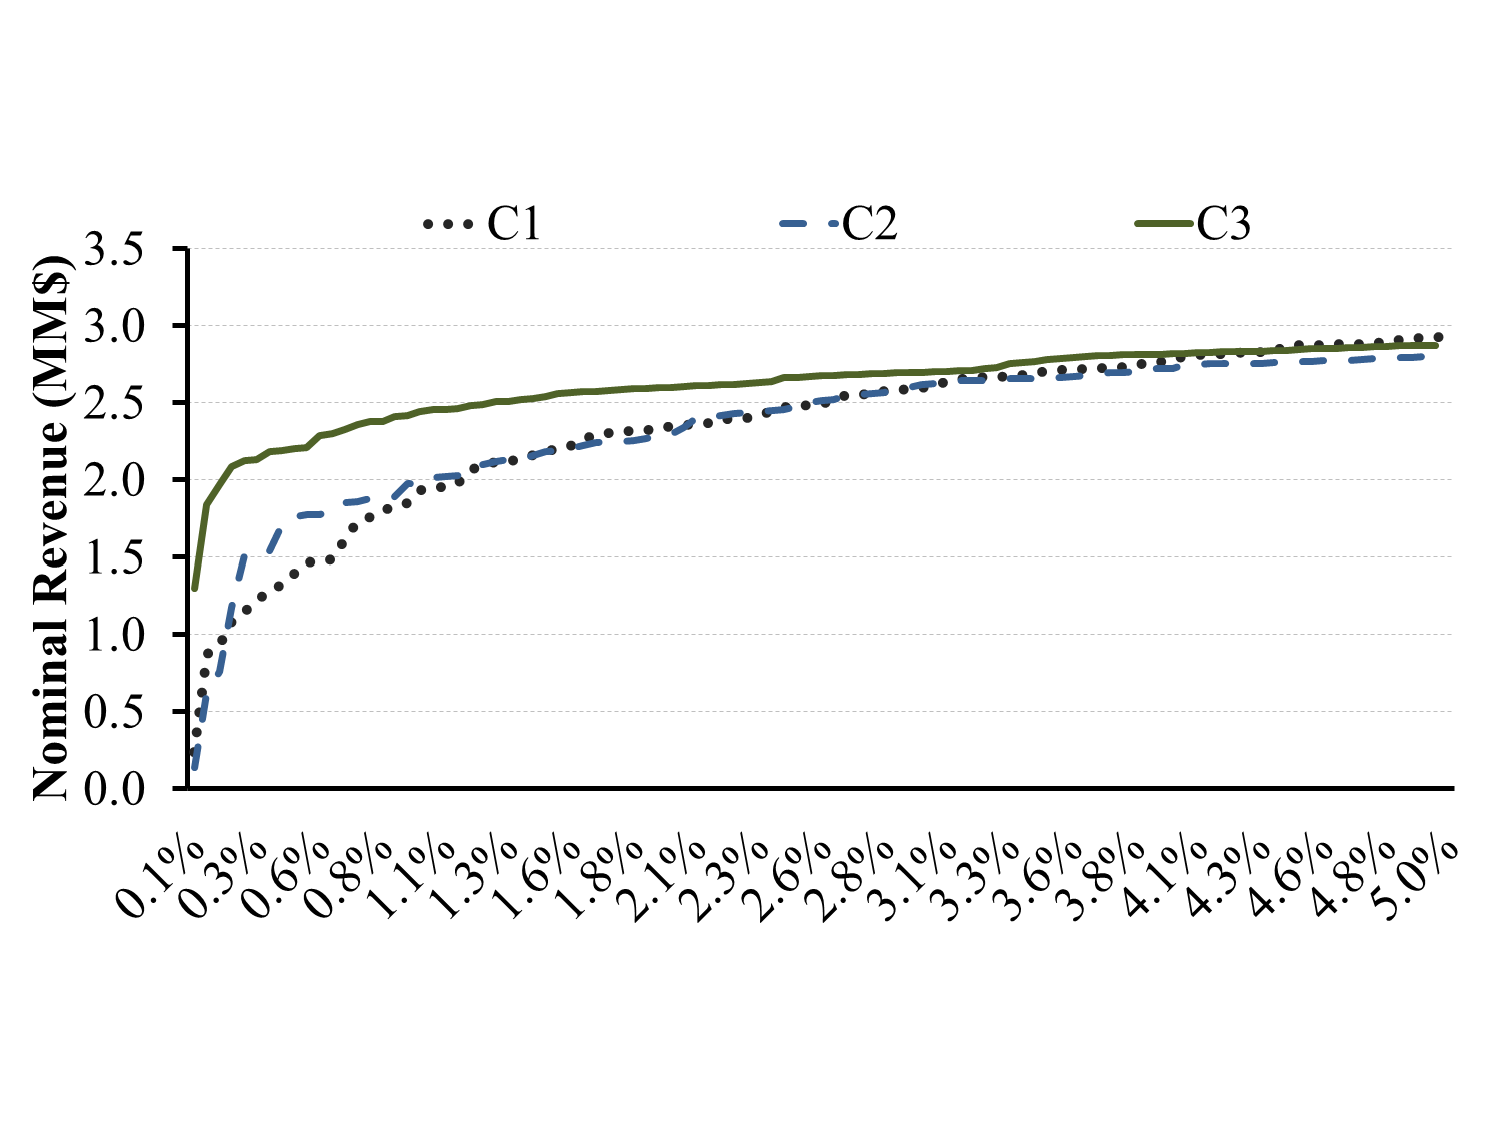
\includegraphics[viewport= 14 98 701 443, clip, width=0.45\textwidth]{./Figures/CurvaPertinencia.pdf}
	\caption{Inverse accumulate probability function restricted to the 5\% worst scenarios of the nominal revenue for the three cases.}
	\label{IAF_CVaR}
\end{figure}
%
\begin{table}
	\renewcommand{\arraystretch}{1.2}
	\centering
	\caption{Expected value of the nominal revenue and $\text{CVaR}_{0.95}$ of the worst-case revenue (MM\$). * identifies a bind constraint.}
	\begin{tabular}{ r | c || c  c  c  c  c  c }
		& & \multicolumn{6}{c}{$\boldsymbol{\text{CVaR}_{0.95}}$} \\
		& $\boldsymbol{\mathbb{E}[\accentset{\sim}{R}]}$ & $\boldsymbol{\accentset{\sim}{R}_{0.5}^{\text{WC}}}$ & $\boldsymbol{\accentset{\sim}{R}_{1.0}^{\text{WC}}}$ & $\boldsymbol{\accentset{\sim}{R}_{1.5}^{\text{WC}}}$ & $\boldsymbol{\accentset{\sim}{R}_{2.0}^{\text{WC}}}$ & $\boldsymbol{\accentset{\sim}{R}_{2.5}^{\text{WC}}}$ & $\boldsymbol{\accentset{\sim}{R}_{3.0}^{\text{WC}}}$ \\
		\hline
		\textbf{C1} & 4.66 & 1.85 & -0.05 & -1.94 & -3.77 & -5.53 & -7.26 \\
		\textbf{C2} & 4.12 & 2.00* & 0.60* & -0.79 & -2.13 & -3.40* & -4.65 \\
		\textbf{C3} & 4.70 & 2.13 & 1.56 & 1.03 & 0.58 & 0.35 & 0.17
	\end{tabular}
	\label{InSample_Analysis}
\end{table}

	In order to validate the proposed methodology, we perform a back test analysis on each of the portfolios against observed data for the uncertain variables. We choose three special years to perform the analysis: (i) 2012, the contract year; (ii) 2010, year where the spot price uncertainty realized as expected (low values in the beginning of the year and high values in the end); (iii) 2008, year in which the observed values of spot price occurred exactly opposite to expected. The financial result of each portfolio in each of the three years is shown in the last three columns of Table \ref{ContractingStrat}. Note that proposed methodology (C2 and C3) outperforms the classical risk-constrained approach (C1) in 2008 and 2012. However, the same performance is not observed in 2010. This result is expected and adequately capture the applicability and relevance of the proposed model with ambiguity treatment. Since the spot price dynamics for 2010 follows a expected pattern, i.e. a pattern explicitly considered in the scenarios used to evaluate the nominal revenue, the classical allocation model (C1) ``optimizes'' the portfolio for the uncertainty environment occurred in 2010. Therefore, the protection imposed by the ambiguity constraints against deviations on the simulated spot scenarios sub-optimizes the portfolio leading to lower gains in 2010. On the other hand, for 2008, a year with observed spot price dynamics different from to the simulated one, the protection created by the ambiguity constraints makes the portfolio allocated by models C2 and C3 to outperform the classical approach C1. Finally, in 2012, we observed atypical spikes in the beginning of the year thus not meeting the expected dynamics of lower prices in this period (bars in Fig. \ref{Backtest_2012}). Therefore, once again, the proposed methodology with ambiguity constraints outperforms the classical one for the same reasons discussed earlier.
%
\begin{figure}[!t]
	\centering
	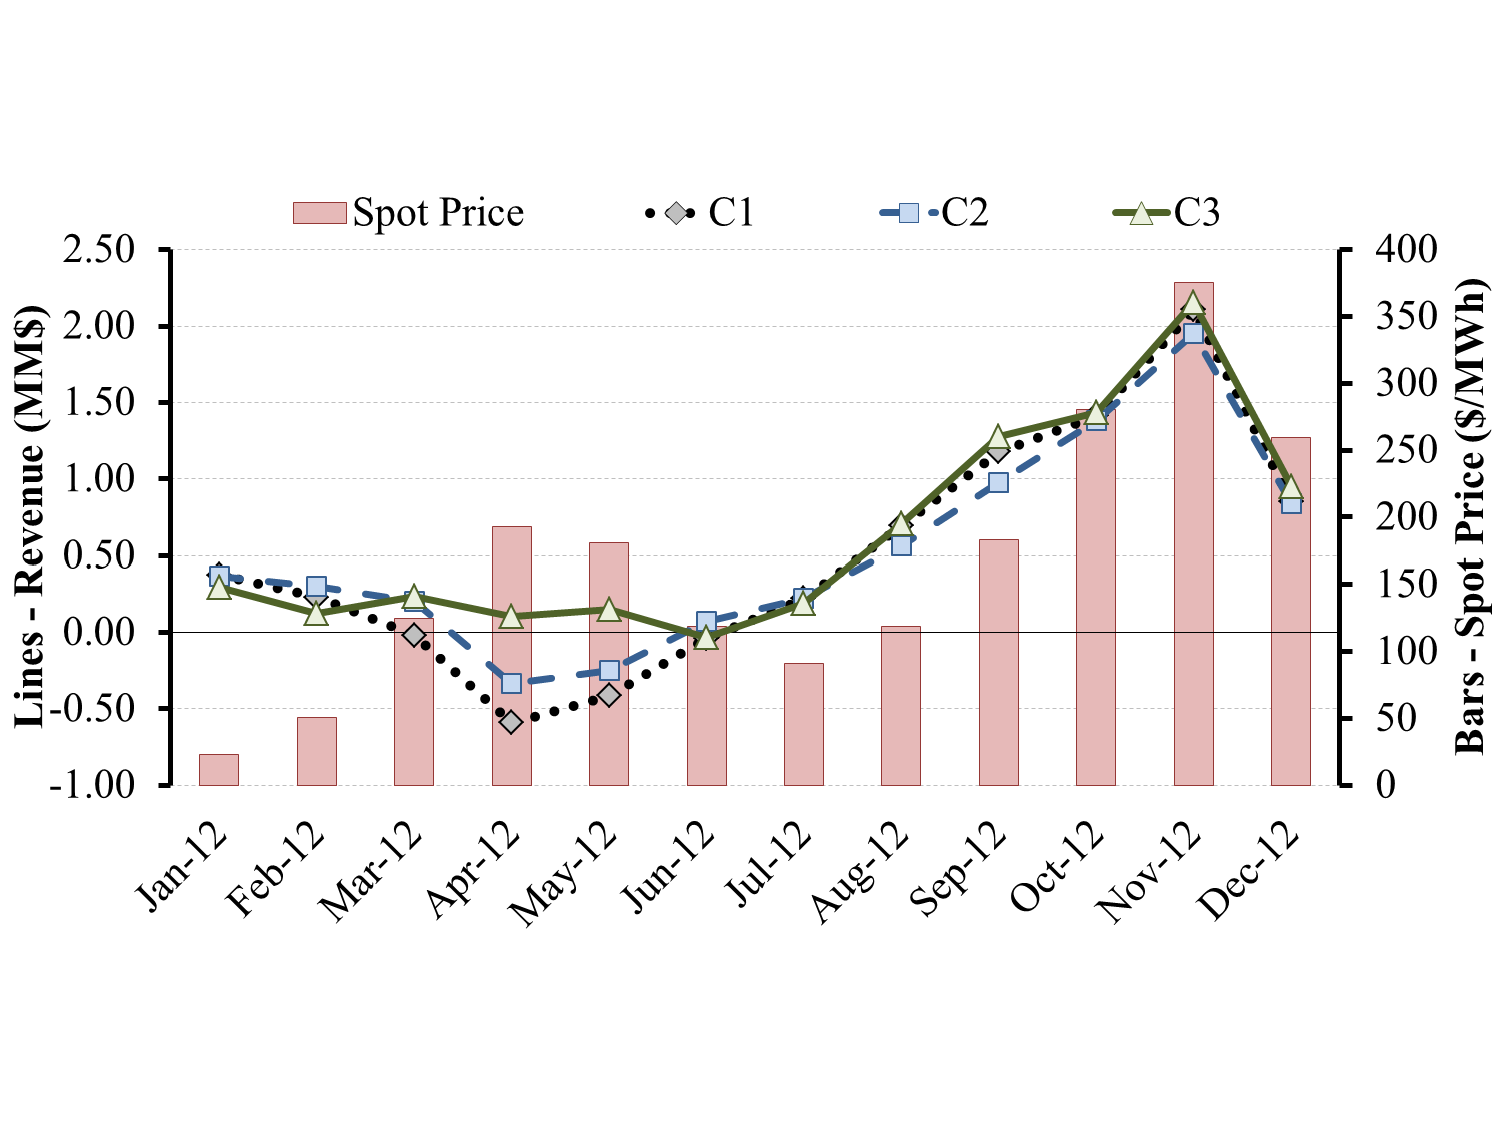
\includegraphics[viewport= 5 95 717 446, clip, width=0.45 \textwidth]{./Figures/BackTest_2012.pdf}
	\caption{Spot prices and revenue profile of the portfolios for the observed data (renewable generation and spot prices) during the contract horizon.}
	\label{Backtest_2012}
\end{figure}

	Finally, to better understand the benefits of the combination of ambiguity constraints and call options, Fig. \ref{Backtest_2012} presents the revenue profile of each portfolio in each month of the contract year. Note that, since the expected pattern of the spot price in the beginning of the years is of low values, without the ambiguity constraints, the set of call options are likely to have no value in the ETC's portfolio. Therefore, if some spikes are observed in this period, as occurred in 2012, the ETC will not be protected. In this context, the ambiguity constraints introduce a robustness in the portfolio allocation that the nominal simulation alone cannot provide. Thus, to protect the portfolio against this ``new'' information, the call options available for the beginning of the year gains value. As a consequence, the revenue of the months of April and May of C3 are strictly positive whereas of C1 and C2 are negative.

% ===== Sec. VI - Conclusion ===== %

\section{Conclusion}
\label{Conclusions}

	In this work, a novel allocation model to optimally assess a portfolio of call options to hedge the price and quantity risk induced by renewable trading in forward market is presented. The proposed approach extend the classical risk-constrained models to include different degrees of aversion to ambiguity on spot price probability distribution. We make use of the hybrid stochastic/robust approach to construct a set of ambiguity constraints to restrict the ETC's trading revenue to minimum profit levels. The benefits of the proposed model is illustrated with real data from the Brazilian system, where the approach presented was contrasted with the classical risk-constrained model and both are benchmarked against historical variables.

% ======================== %

%\section*{Acknowledgment}

%The authors would like to thank FICO (Xpress-MP developer) for the academic partnership program with the Electrical Engineering Department of Pontifical Catholic University of Rio de Janeiro, Brazil (PUC-Rio). The authors would also like thank the LAMPS researchers for the daily exchanges and their insightful considerations.

%\IEEEtriggeratref{17}
\bibliographystyle{IEEEtran}
\bibliography{Bibliography}

%\begin{IEEEbiographynophoto}{Bruno Fanzeres} (S'11) has a B.Sc. degree in Electrical and Industrial Engineering and a M.Sc. degree in Operations Research from PUC-Rio, Brazil. He is pursuing a Ph.D degree in Operations Research at the same university.
%\end{IEEEbiographynophoto}

%\begin{IEEEbiographynophoto}{Arthur Brigatto} (S'14) received a B.Sc. degree in Electrical Engineering from the Federal University of Juiz de Fora, Brazil, and is pursuing a M.Sc. in Electrical Engineering at PUC-Rio, Brazil.
%\end{IEEEbiographynophoto}

%\begin{IEEEbiographynophoto}{Alexandre Street} (S'06, M'10) holds the degrees of M.Sc. and D.Sc. in Electrical Engineering (Operations Research) from PUC-Rio, Brazil. 
%\end{IEEEbiographynophoto}

%\begin{IEEEbiographynophoto}{Luiz Augusto Barroso} (S'00, M'06, SM'07) has a B.Sc. in Mathematics and a Ph.D degree in Operations Research. He is a technical director at PSR.
%\end{IEEEbiographynophoto}

\end{document}
